\section{Implementation Plan}
The implementation of Data4Help and AutomatedSOS systems is carried on taking into consideration some important factors, such as the complexity of each component and its relations with the others. Of course, the implementation plan takes into special consideration the core components which are essential for the whole system and are considered as \say{bottleneck}. 
It is important to fix any flaw as soon as it is detected, so that the correction cost in terms of time is kept the lowest possible.
The order in which our system is implemented is the following:

\begin{enumerate}
    \item Model
    \item Central Controller
    \item Account Manager
    \item Third party services, User Services
    \item Emergency Service
    \item Web, Mobile and Wearable Applications
\end{enumerate}
\begin{figure}[H]
    \makebox[\textwidth]{
        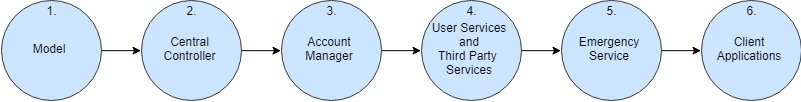
\includegraphics[width=1.3\linewidth]{images/Implementation_plan.png}
    }
\end{figure}

\subsubsection{Model}
The Model is the first step of the implementation plan, according to its vital role for the whole application.
Since the classes of the Model are used by all the components, it is important that they are ready as soon as possible to be used as a reference. Otherwise each team member would implement the classes of the Model \say{on the fly} when he/she needs them, introducing possible implementation flaws or not using abstraction in a proper way.

\subsubsection{Central Controller}
This component is the logic core of the application. According to this, it requires lot of time to be implemented and, consequently, it is a risky component. It is important that the least possible flaws are inserted during its implementation, since they may have catastrophic consequences in terms of time costs.\\
An important non functional requirement for the Central Controller is the fault-tolerance and the high throughput. This component may be stressed by lots of requests from users and third party, so it has to react in a short time. For this reason, this component is consider as a \say{bottleneck}.

\subsubsection{Account Manager}
This module allows the sign-up and login of the users and third parties and is also used by the Central Controller when a third party composes a request for data of a specific user. As shown in the \hyperlink{RV}{\underline{Runtime view, section 2.5}}, the third party fills the request form specifying the user's SSN or Fiscal Code and, thanks to the Account Manager, the Central Controller converts it into the corresponding user ID.
This module is used by different kind of clients and, consequently, it has to use abstraction to interact with all of them.

\subsubsection{Third party services, User Services}
These two components allow the interaction between the user application (mobile or wearable) and the third party application (mobile or web), passing through the Central Controller.
They can be implemented together, since they are quite similar to each other.
As shown in the \hyperlink{CV}{\underline{Component view, section 2.5}}, the sub-components that allows the login, the registration and the access to data are present in both modules.
Regarding to the Individual and the Group requests, the Third party services component offers the possibility to create them while the User services component allow the user to manage them.
According to what just said, they are implemented just after the Central Controller and the Account Manager.

\subsubsection{Emergency Service}
This component has a vital role for the AutomatedSOS system. It analyzes real-time health parameters by comparing them with specific thresholds. It is strictly dependent on the User services component and on the Central Controller, so it has to be implemented after they are ready to use.
Of course, the Emergency Service has to be fault tolerant since it deals with human lives. In case of failure of this component, the error must be repaired as soon as possible since the system must result available 24/7. 
This component must guarantee an high throughput since it receives a large amount of real-time health data from all the users at the same time.

\subsubsection{Web, Mobile and Wearable Applications}
The remaining elements of the system to be implemented are the client applications. They allow users and third parties to interact with the system, but they don't contain core logic functions of the system.
They represent only a minimum part of the code and they require a short time to be implemented. 
The web apps must be compatible with all the major browsers, while the mobile apps must be developed for Android and iOS platforms.
The applications must properly run on different devices both for the users (smart-phones and wearable-devices) and the third parties (personal computers, tablets and smart-phones).\\
For these reasons, client components are not considered \say{risky} and they are taken into account as the last part of the implementation plan.

\clearpage
\section{Integration and Testing}
\subsection{Entry Criteria}
Integration testing is an important process that has to start as soon as every component is almost complete, in order to promptly fix any flaw that could eventually occur. \\
The purpose of this process is to test the integration between the components of our system, according to all the functionalities listed in the RASD and the DD documents that our application will be able to offer. \\
To start the Integration each component has to correctly pass its unit test.
All the services provided by external entities, including each APIs (Google Maps API and the APIs of the health sensors), have to be completed and they have to properly work since our system will heavily depends on them. For the same reason, also the DBMS and the Data Manager service must be completed before starting all tests. \\
Regarding the AutomatedSOS system-to-be, we have already explained how the interaction between the system and the National Health Services can change according the host country. In the nations in which the NHS provides an API, the latter must be completed before starting the integration tests. Otherwise, there must be an operative VoIP API that allows AutomatedSOS to interact with the NHS.\\ \\
The integration process between two components should start when both of them have reached a minimum level of completion, in order to make the integration tests meaningful.\\
To be detailed, the estimated completion of each component to enter the integration process should be:
\begin{itemize}
    \item Data Manager, \textbf{100\% of completion}
    \item Central Controller, \textbf{90\% of completion}
    \item Account Manager, \textbf{70\% of completion}
    \item Third Party Services, \textbf{60\% of completion}
    \item User Service, \textbf{60\% of completion}
    \item Emergency Services, \textbf{80\% of completion}
    \item Third Party Client Applications, \textbf{40\% of completion}
    \item User Client Applications, \textbf{40\% of completion}
\end{itemize}
In the bulleted list above, the percentages reflect the minimum number of functions that each component must offer in order to enter the integration process.
\clearpage

\subsection{Elements to be Integrated}
As already mentioned in the \hyperlink{SOA_TG}{\underline{Architectural Patterns section}}, the system is based on a Service Oriented Architecture, which guarantees the modularity and the maintainability of the software. Each component offers some interfaces to communicate with the others.
It's important to test the integration of the modules to ensure the reliability of the system. \\
Moreover, each requirement listed in the RASD document is achieved through the numerous interactions between the interfaces of all the components.\\
We identify four different macro-categories in which components can be grouped, according to their role inside the system.
Referring to the high-level components in the Figure \underline{\ref{HLC}}, these categories are:
\begin{itemize}
    \item Client components: third party web application, user mobile application, user wearable application.
    \item Logic components: Third party services, user services, account manager, central controller, emergency services.
    \item Data components:  data manager, DBMS.
    \item External components: Maps API, VoIP API, Sensors API.
\end{itemize}
This separation facilitates us in the process of the integration. 
The Logic category represents the core of the application, so the majority of the interactions takes place inside this group.
On the contrary, there aren't interactions between components inside the Client categories.\\
In the following lines we list all the elements that need to be integrated together, belonging to the same or to different categories.\\ \\
\textbf{Integration of Logic Components with Data and External components:}
\begin{itemize}
    \item Central Controller
    \begin{itemize}
        \item Data Provider, Data Manager
        \item Data Gatherer, Data Manager
    \end{itemize}
    \item User Services
    \begin{itemize}
        \item Data Acquisition Manager, Sensors API
        \item Access to Data, Maps API
    \end{itemize}
    \item Third Party Services
    \begin{itemize}
        \item Group Request Service, Maps API
        \item Access to Data, Maps API
    \end{itemize}
    \clearpage
    \item Emergency Service
    \begin{itemize}
        \item Data Analyzer, Data Manager
        \item NHS Adapter, NHS API
    \end{itemize}
\end{itemize}

\textbf{Integration between Logic Components:}
\begin{itemize}
    \item Central Controller
    \begin{itemize}
        \item Individual Request Manager, Requests Manager (User Services)
        \item Individual Request Manager, Notification Manager (User Services)
    \end{itemize}
    \item User Services
    \begin{itemize}
        \item Data Sending Service, Data Gathering (Central Controller)
        \item Login Service, Account Manager
        \item Registration Service, Account Manager
    \end{itemize}
    \item Third Party Services
    \begin{itemize}
        \item Individual Request Service, Individual Request Manager (Central Controller)
        \item Group Request Service, Group Request Manager (Central Controller)
        \item Access to Data, Data Provider (Central Controller)
        \item Login Service, Account Manager
        \item Registration Service, Account Manager
    \end{itemize}
    \item Emergency Service
    \begin{itemize}
        \item Data Analyzer, Data Provider (Central Controller)
        \item Emergency Manager, Account Manager (Central Controller)
        \item User Communication Manager, Notification Manager (User Services)
    \end{itemize}
\end{itemize}

\textbf{Integration of Client Components with Logic Components:}
\begin{itemize}
    \item User Web, Mobile and Wearable Applications, User Services
    \item Third Party Web and Mobile Applications, Third Party Services
\end{itemize}

\clearpage
\subsection{Integration Testing Strategy}
According to the implementation plan stated before, we decided to integrate the components using a mixture of two strategies: the \textbf{Bottom Up} and the \textbf{Critical Module First}.\\
The \textbf{Bottom Up} approach allows us to test the ready components directly in a real world scenario, avoiding the creation of stubs. It's important that the external services are available for the integration process from the beginning.\\
As soon as a component or a part of it has been implemented, it can be integrated with the already existing ones which lies in the lower levels of the hierarchy. Using this method we are able to find out the behavior of the system in the real world usage, and we can promptly intervene if something goes wrong.\\
Also, we chose this integration approach to optimize the efficiency of the development, since it reflects the same approach used during the implementation phase.
Components that lies in the same hierarchy level can be integrated in an arbitrary order, maybe integrating the ones that are ready first.\\
The Logic components represent the core of the entire system, so it is necessary to start integrating them from the beginning.
For this reason we also decided to use the \textbf{Critical Module First} approach to start integrating the riskiest components first.
Since a fault in these components may have tragic consequences for the entire system, this approach allows us to fix the bugs earlier.\\
Components provided by external entities, such as \textbf{Maps API}, \textbf{health sensors APIs}, \textbf{NHS API} and \textbf{VoIP API} can be immediately used in the integration since we assume that they are ready before all the others. Also the \textbf{Data Manager} and the \textbf{DBMS} components have to be completed before starting the integration, since the lower level of the hierarchy strongly depends on them.\\
\subsection{Sequence of Component/Function Integration}
This section illustrates the integration of components in our systems. The following diagrams represent the order that will be followed during the process. An arrow going from component X to component Y means that Y is necessary for X functioning, so it must have already been implemented before the integration happens.

\subsubsection{Software Integration Sequence}
Following a bottom-up approach, the integration process will start by connecting the submodules of the system.
In the first step we will focus on the integration of logic components with data and external components, then we will proceed with the integration of subcomponents in the central logic.
\clearpage
\noindent\textbf{Integration of Logic Components with Data Components:}
the first step in the sequence will concern the integration of the back-end submodules with the data management system. We chose to start from here because of the data-centric nature of the applications. As it's possible to see in the diagrams below, several submodules rely on a correct communication with the Data Manager.

\begin{figure}[H]
    \centering
    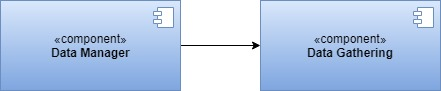
\includegraphics[width=295pt]{images/IntegrationSequence/TrackMe-Integration_sequence2.jpg}
    \caption{Integration of the Data Gathering and the Data Manager.}
\end{figure}
\begin{figure}[H]
    \centering
    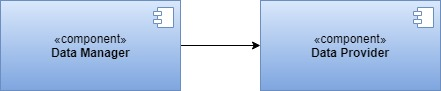
\includegraphics[width=295pt]{images/IntegrationSequence/TrackMe-Integration_sequence1.jpg}
    \caption{Integration of the Data Provider and the Data Manager.}
\end{figure}
\begin{figure}[H]
    \centering
    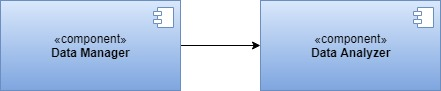
\includegraphics[width=295pt]{images/IntegrationSequence/TrackMe-Integration_sequence7.jpg}
    \caption{Integration of the Data Analyzer and the Data Manager.}
\end{figure}

\noindent\textbf{Integration of Logic Components with External Components:} the second step will be devoted to the integration with APIs provided by external entities. These components often play an essential role in the success of the system and it's important to test their functioning as soon as possible, in order to be able to react to eventual faults.
\begin{figure}[H]
    \centering
    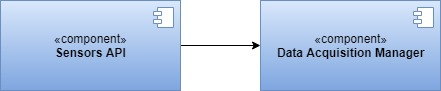
\includegraphics[width=295pt]{images/IntegrationSequence/TrackMe-Integration_sequence3.jpg}
    \caption{Integration of the Data Acquisition Manager and the Sensors API.}
\end{figure}
\begin{figure}[H]
    \centering
    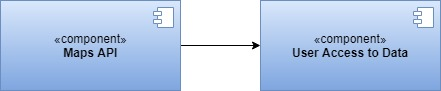
\includegraphics[width=295pt]{images/IntegrationSequence/TrackMe-Integration_sequence4.jpg}
    \caption{Integration of the User Access to Data and the Maps API.}
\end{figure}
\begin{figure}[H]
    \centering
    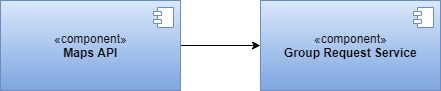
\includegraphics[width=295pt]{images/IntegrationSequence/TrackMe-Integration_sequence5.jpg}
    \caption{Integration of the Group Request Service and the Maps API.}
\end{figure}
\begin{figure}[H]
    \centering
    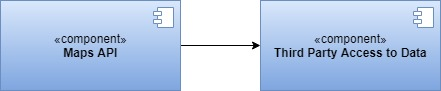
\includegraphics[width=295pt]{images/IntegrationSequence/TrackMe-Integration_sequence6.jpg}
    \caption{Integration of the Third Party Access to Data and the Maps API.}
\end{figure}
\begin{figure}[H]
    \centering
    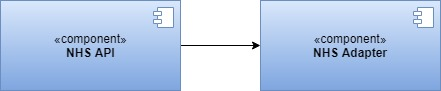
\includegraphics[width=295pt]{images/IntegrationSequence/TrackMe-Integration_sequence8.jpg}
    \caption{Integration of the NHS Adapter and the NHS API.}
\end{figure}
\begin{figure}[H]
    \centering
    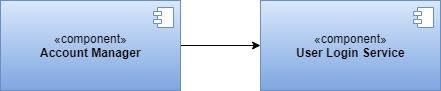
\includegraphics[width=295pt]{images/IntegrationSequence/TrackMe-Integration_sequence20.jpg}
    \caption{Integration of the NHS Adapter and the VoIP API.}
\end{figure}
\clearpage
\noindent\textbf{Integration between Logic Components:} the third step will be devoted to the integration of all the subcomponents in the back-end. This phase will be the longest and most complex of the process, given the great number of interactions that happens between the logic components. \\
For these reasons, the sequence of integration will follow a Critical Module First approach: initially, we will integrate the subcomponents regarding the collection and the exchange of data between the parties; then we will move on to connect the modules that deal with the account credentials and the dispatch of notifications.
\begin{figure}[H]
    \centering
    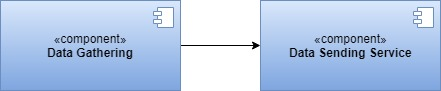
\includegraphics[width=295pt]{images/IntegrationSequence/TrackMe-Integration_sequence10.jpg}
    \caption{Integration of the Data Sending Service and the Data Gathering.}
\end{figure}
\begin{figure}[H]
    \centering
    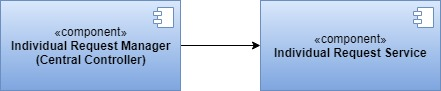
\includegraphics[width=295pt]{images/IntegrationSequence/TrackMe-Integration_sequence13.jpg}
    \caption{Integration of the Individual Request Service and the Individual Request Manager.}
\end{figure}
\begin{figure}[H]
    \centering
    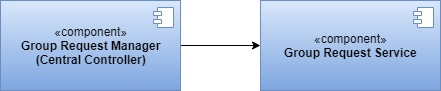
\includegraphics[width=295pt]{images/IntegrationSequence/TrackMe-Integration_sequence14.jpg}
    \caption{Integration of the Group Request Service and the Group Request Manager.}
\end{figure}
\begin{figure}[H]
    \centering
    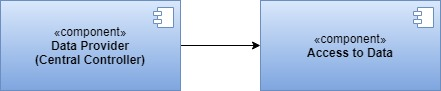
\includegraphics[width=295pt]{images/IntegrationSequence/TrackMe-Integration_sequence15.jpg}
    \caption{Integration of the Third Party Access to Data and the Data Provider.}
\end{figure}
\begin{figure}[H]
    \centering
    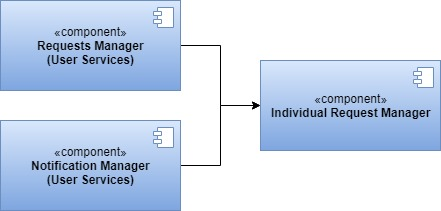
\includegraphics[width=295pt]{images/IntegrationSequence/TrackMe-Integration_sequence9.jpg}
    \caption{Integration of the Individual Request Manager and the Requests and Notification Managers}
\end{figure}
\begin{figure}[H]
    \centering
    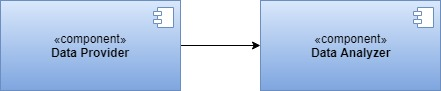
\includegraphics[width=295pt]{images/IntegrationSequence/TrackMe-Integration_sequence18.jpg}
    \caption{Integration of the Data Analyzer and the Data Provider.}
\end{figure}
\begin{figure}[H]
    \centering
    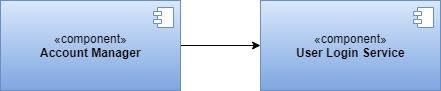
\includegraphics[width=295pt]{images/IntegrationSequence/TrackMe-Integration_sequence11.jpg}
    \caption{Integration of the User Login Service and the Account Manager.}
\end{figure}
\begin{figure}[H]
    \centering
    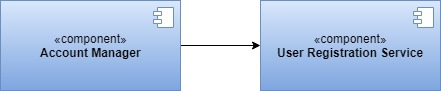
\includegraphics[width=295pt]{images/IntegrationSequence/TrackMe-Integration_sequence12.jpg}
    \caption{Integration of the User Registration Service and the Account Manager.}
\end{figure}
\begin{figure}[H]
    \centering
    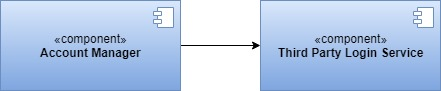
\includegraphics[width=295pt]{images/IntegrationSequence/TrackMe-Integration_sequence16.jpg}
    \caption{Integration of the Third Party Login Service and the Account Manager.}
\end{figure}
\begin{figure}[H]
    \centering
    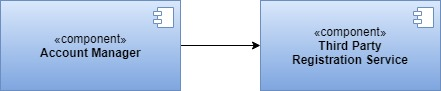
\includegraphics[width=295pt]{images/IntegrationSequence/TrackMe-Integration_sequence17.jpg}
    \caption{Integration of the Third Party Registration Service and the Account Manager.}
\end{figure}
\begin{figure}[H]
    \centering
    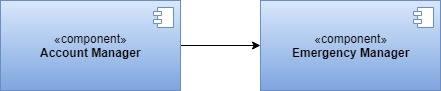
\includegraphics[width=295pt]{images/IntegrationSequence/TrackMe-Integration_sequence19.jpg}
    \caption{Integration of the Emergency Manager and the Account Manager.}
\end{figure}
\begin{figure}[H]
    \centering
    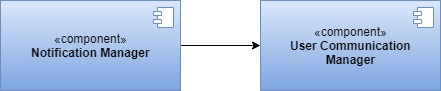
\includegraphics[width=295pt]{images/IntegrationSequence/TrackMe-Integration_sequence21.jpg}
    \caption{Integration of the User Communication Manager and the Notification Manager.}
\end{figure}
\clearpage
\subsubsection{Subsystem Integration Sequence}
Once all the submodules will be connected, we will proceed with the integration of the high level components, resulting in the final and complete system.
In the final phase we will integrate the back-end system to the various instances of the presentation layer: web, mobile and wearable applications.\\
The following diagram gives an overview of the dependencies between the high level components, highlighting the sequence of integration that composes the system from the data layer to the client applications. 
\begin{figure}[H]
    \makebox[\textwidth]{
        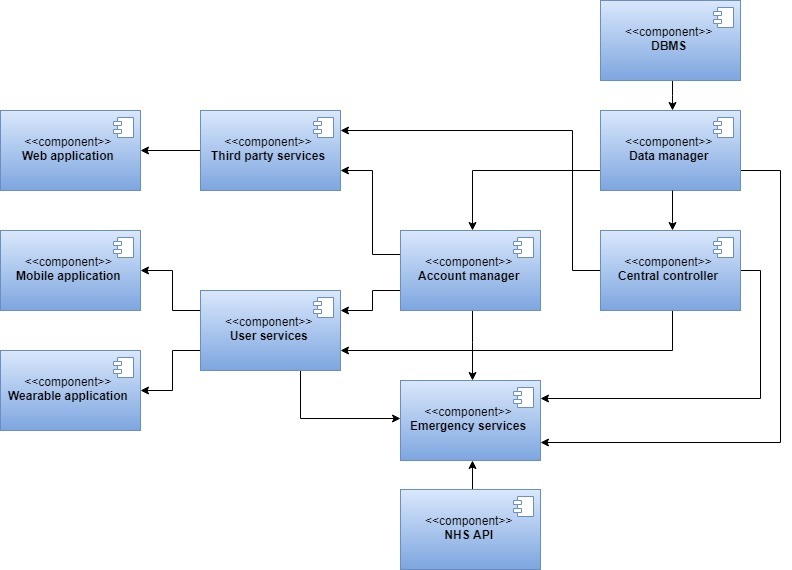
\includegraphics[width=1.4\linewidth]{images/IntegrationSequence/Subsystem_Integration_sequence.jpg}
    }
\end{figure}